\section{Comunicazione dati}
    Ci interessa, per una serie di motivi, poter scambiare dati fra due qualsiasi parti del mondo, in qualsiasi momento, e possibilmente con una velocità e accuratezza quanto più alte possibile.
    
    Il termine \textbf{comunicazione dati} fa riferimento allo scambio di dati fra due dispositivi che fanno parte dello stesso sistema di comunicazione, e collegati da un mezzo, come un cavo. Questo sistema di comunicazione dipende da quattro caratteristiche fondamentali:
    \begin{itemize}
        \item \textbf{Consegna.} Il sistema deve essere in grado di consegnare i dati al destinatario corretto e solo a lui.
        
        \item \textbf{Precisione.} Il sistema deve consegnare i dati senza alterarli durante la trasmissione.
        
        \item \textbf{Tempestività.} Talvolta i dati arrivati in ritardo sono inutili. In alcuni casi i dati devono arrivare in maniera tempestiva e nell'ordine in cui sono stati spediti, come nello streaming video. Questo tipo di comunicazione si dice in \textit{tempo reale}.
        
        \item \textbf{Jitter.} Questo termine si riferisce alla variazione del ritrardo con cui arrivano i dati. Se per esempio alcuni pacchetti dati arrivano con un ritardo di 30ms e altri con un ritardo di 40ms, potremmo avere una riproduzione a scatti.
    \end{itemize}
    
    \subsection{Componenti}
        Un sistema di comunicazioni ha cinque componenti:
        \begin{itemize}
            \item \textbf{Messaggio.} I dati che devono essere inviati. Possono assumere varie forme con rappresentazioni e caratteristiche diverse.
            
            \item \textbf{Mittente.} Il dispositivo che spedisce il messaggio. Anche questo può essere soggetto a variazione.
            
            \item \textbf{Destinatario.} Il dispositivo che riceve il messaggio.
            
            \item \textbf{Mezzo di trasmissione.} È il mezzo fisico di comunicazione sul quale il messaggio viene spedito dal mittente per raggiungere il destinatario. Alcune delle forme che può assumere sono onde elettromagnetiche, cavi di rame, fibre ottiche.
            
            \item \textbf{Protocollo.} Una serie di regole che governano la trasmissione e che sono state adottate dai dispositivi ai due capi della comunicazione. Senza un protocollo due dispositivi potrebbero riuscire a connettersi ma non a comunicare.
        \end{itemize}
        
    \subsection{Rappresentazione dei dati}
        Tipi di dati quali \textbf{immagini}, \textbf{numeri},  \textbf{testo} e qualsiasi altra informazione in forma discreta, sono rappresentati da sequenze di bit, ognuna in un formato opportuno e spesso più di uno stesso formato per lo stesso tipo di dato (per esempio jpeg e png per le immagini).
        
        Tipi di informazione come \textbf{audio} e \textbf{video} sono per natura non discreti. Va trovato quindi il modo per rappresentarli (convertirli) in un formato discreto, adatto a essere rappresentato da una sequenza di bit.
        
    \subsection{Flusso di dati}
        La comunicazione fra due dispositivi può essere di tre tipi: unidirezionale, bidirezionale alternata e bidirezionale.
        
        Nella modalità \textbf{unidirezionale}, o \textit{simplex}, uno solo dei dispositivi può ricevere i dati, mentre l'altro può solo inviarli. Si pensi a una tastiera o un monitor. In questa modalità l'intera capacità del canale può essere sfruttata per il trasferimento dei dati.
        
        Nella comunicazione \textbf{bidirezionale alternata}, o \textit{half-duplex}, entrambi i dispositivi possono inviare o ricevere dati, ma non contemporaneamente. Quando un dispositivo invia dati, l'altro deve ricevere e viceversa. Un esempio sono le radio ricetrasmittenti, e anche qui l'intera capacità del canale può essere sfruttata per inviare dati.
        
        Abbiamo infine la comunicazione \textbf{bidirezionale}, o \textit{full-duplex}, nella quale ogni dispositivo può inviare e ricevere dati, anche contemporaneamente, come per esempio in una conversazione telefonica. In questo caso la capacità del canale deve essere divisa fra i due dispositivi.
        
\section{Reti}
    Una rete è un insieme di dispositivi (nodi) connessi da canali di comunicazione. Un nodo può essere un computer o qualsiasi altro dispositivo capace di spedire o ricevere dati. Uno dei vantaggi di questo tipo di organizzazione è il calcolo distribuito.
    
    \subsection{Criteri di valutazione}
        Fra i criteri più importanti abbiamo i seguenti tre:
        \begin{itemize}
            \item \textbf{Prestazioni.} Possono essere misurate in vari modi, per esempio tramite il tempo di risposta o il ritardo.
            Le metriche spesso utilizzate sono il \textbf{throughput}, ossia la quantità di dati che si riesce effettivamente a spedire nell'unità di tempo, e il \textbf{ritardo}, ossia il tempo necessario a un messaggio per viaggiare dalla sorgente alla destinazione. Chiaramente si vuole massimizzare il throughput e minimizzare il ritardo, ma altrettanto chiaramente questi obiettivi sono in contrasto fra di loro in quanto più dati si inviano sulla rete, più questi viaggiano lentamente, causa congestione del traffico.
            
            \item \textbf{Affidabilità.} È determinata dalla capacità della rete di inviare dati senza errori, ma viene combinata alla sua resistenza ai guasti, alla sua robustezza in casi limite, etc.
            
            \item \textbf{Sicurezza.} Include la protezione dei dati che viaggiano sulla rete stessa, la quale impedisce accesso non autorizzato, danni o perdite dovute a violazioni della rete.
        \end{itemize}
        
    \subsection{Struttura fisica}
        Per proseguire nella discussione occorre definire alcuni dettagli sulla struttura e sulla topologia delle reti.
        
        \subsubsection{Tipo di connessione}
            Le connessioni che collegano due punti in una rete possono essere classificate in due categorie: connessione punto-punto e connessione multipunto.
            
            Una connessione \textbf{punto-punto} si ottiene dedicando un canale fisico ai due dispositivi che devono comunicare. Ogni volta che colleghiamo due dispositivi tramite un cavo si ottiene questo tipo di connessione. Il vantaggio è che l'intera capacità del canale è dedicata alla comunicazione dei due dispositivi.
            
            Una connessione \textbf{multipunto} invece, prevede il collegamento di più di due dispositivi a un canale di comunicazione, chiaramente dividendo la sua capacità su tutti i dispositivi connessi. I dispositivi potrebbero potersi connettere contemporaneamente o a turno.
            
            \begin{figure}[h]
                \centering
                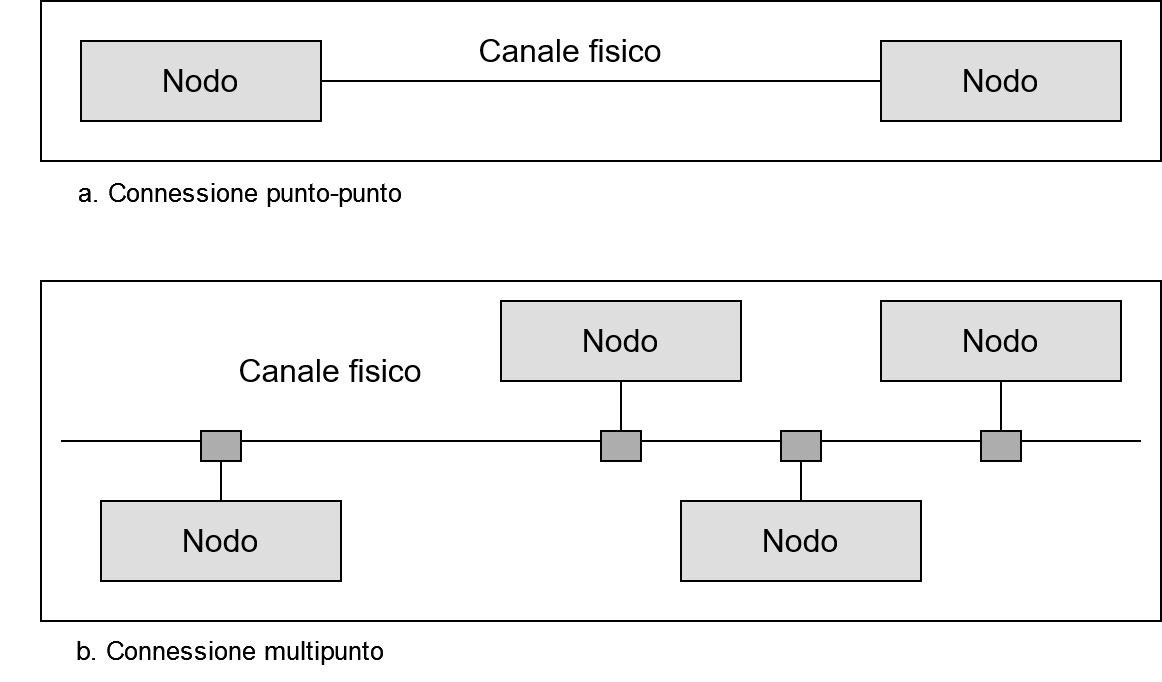
\includegraphics[width=0.8\textwidth]{img/img1.png}
                \caption{Differenza fra connessione punto-punto e multipunto.}
                \label{fig:img1}
            \end{figure}
            
        \newpage
        \subsubsection{Topologia}
            La topologia di una rete è il modo in cui i nodo sono fisicamente disposti e interconnessi. Essa è descritta dalla disposizione dei collegamenti, e quindi dei nodi, della rete. Esistono quattro tipi di topologie di base: mesh, stella, bus e anello.
            
            \paragraph{Mesh} In questa topologia ogni nodo ha un collegamento punto-punto con ogni altro nodo della rete. Il numero di collegamenti è quadratico nel numero dei nodi, sia usando collegamenti simplex che duplex.
            
            Le reti mesh sono usate con parsimonia, in quanto la manutenzione e l'installazione di nuovi nodi risultano dispendiose, a causa del grande numero di cavi.
            
            I vantaggi sono invece la grande interconessione; se un singolo collegamento diventa inusabile, ci sono molti altri cammini per trasferire i dati da un nodo all'altro. Questo chiaramente aumenta l'affidabilità e la sicurezza. Tuttavia dobbiamo notare che se un nodo è usato come punto di passaggio per parecchi cammini dati, il suo guasto potrebbe portare molti disagi.
            
            \begin{figure}[h]
                \centering
                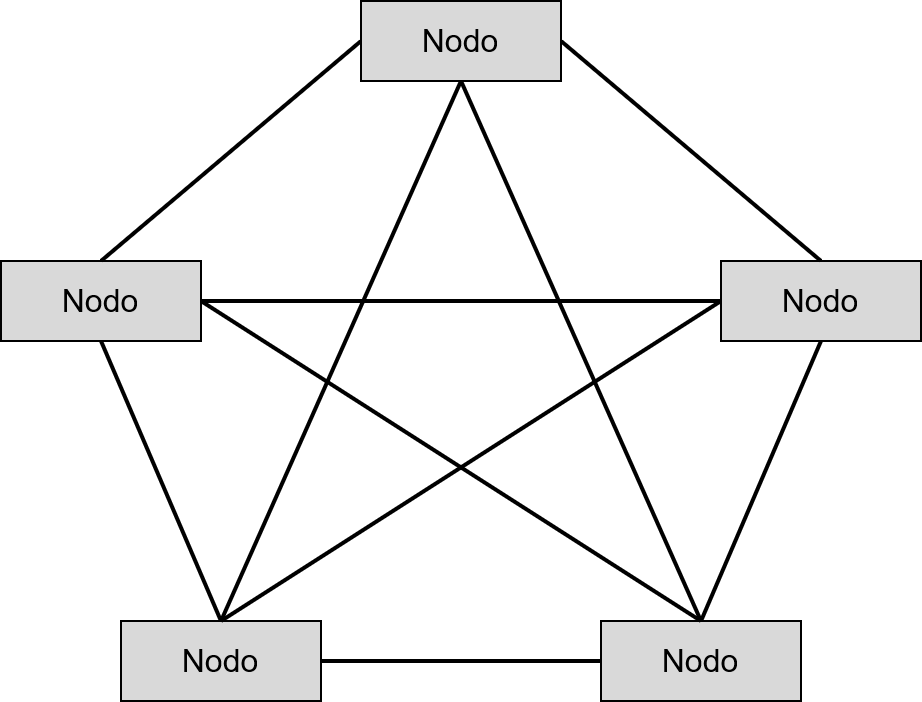
\includegraphics[width=0.45\textwidth]{img/mesh.png}
                \caption{Topologia mesh.}
                \label{fig:img1}
            \end{figure}
            
            \paragraph{Stella} Nella topologia a stella, ogni nodo è connesso tramite un collegamento punto-punto a un dispositivo centrale chiamato \textbf{hub}. Al contrario della topologia mesh, i nodi non possono essere in collegamento diretto fra di loro.
            
            Il vantaggio principale sta nel costo e nella manutenzione, in quanto il numero di porte I/O e collegamenti è lineare rispetto al numero dei nodi.
            
            Lo svantaggio principale sta nella presenza dell'hub, in quanto un suo guasto rischia di compromettere l'intera rete. Potrebbe inoltre fungere da collo di bottiglia per le prestazioni.
            
            \begin{figure}[h]
                \centering
                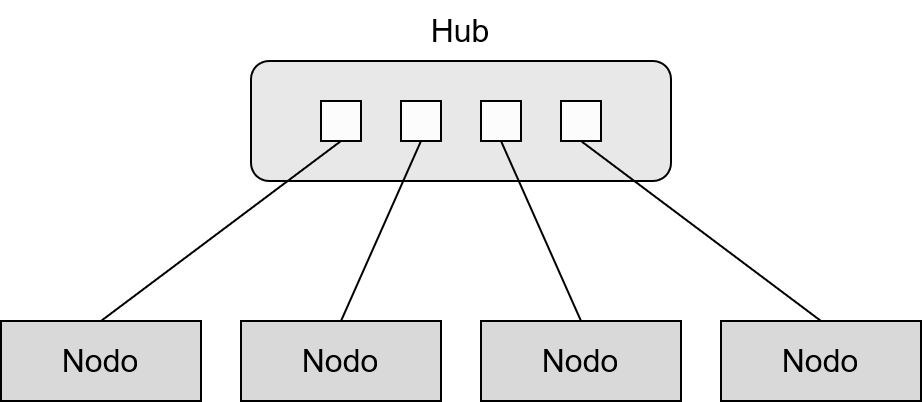
\includegraphics[width=0.55\textwidth]{img/stella.png}
                \caption{Topologia a stella.}
                \label{fig:img1}
            \end{figure}
            
            \newpage
            \paragraph{Bus} Questo tipo di rete utilizza un collegamento multipunto (il bus) che collega tutti i nodi della rete.
            
            Il problema principale è che il segnale diminuisce d'intensità attraversando il bus, e quindi questo non può essere molto lungo e quindi non può ospitare un grande numero di nodi.
            
            Il vantaggio principale sta nella semplice aggiunta di un nuovo nodo, che consta semplicemente nell'aggiunta di un connettore al bus. Tuttavia i nodi devono essere opportunamente distanziati e non creare rumore sul bus.
            
            \begin{figure}[h]
                \centering
                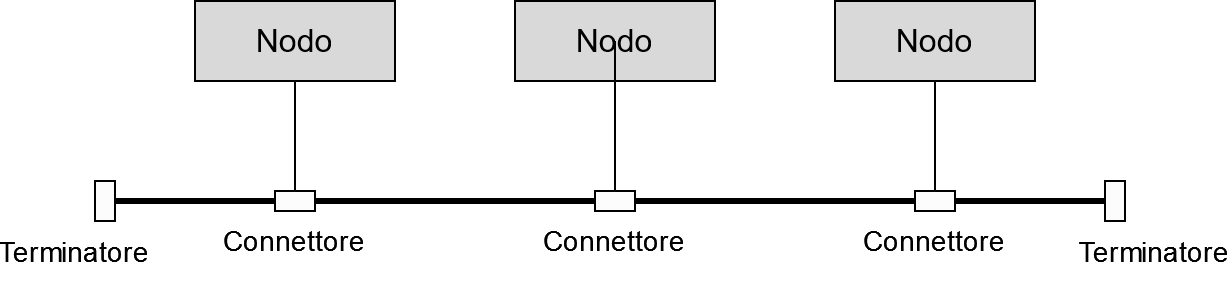
\includegraphics[width=0.70\textwidth]{img/bus.png}
                \caption{Topologia bus.}
                \label{fig:img1}
            \end{figure}
            
            \paragraph{Anello} In una tale topologia ogni nodo ha un collegamento punto-punto con soli altri due nodi: quello che lo segue e quello che lo precede nell'anello.
            
            I dati vengono fatti passare sull'anello in una sola direzione, e ogni anello ha un ripetitore che rigenera il segnale fino a che questo raggiunge la sua destinazione.
            
            La manutenzione e l'aggiunta di un nodo risultano abbastanza semplici. Quest'ultima richiede la modifica di due sole connessioni, quella precedente rispetto al nodo da aggiungere e quella successiva.
            
            Lo svantaggio principale sta nella natura unidirezionale della topologia: il guasto di un singolo collegamento rende non funzionante l'intera rete. Si può ovviare a questo problema usando un doppio anello.
            
            \begin{figure}[h]
                \centering
                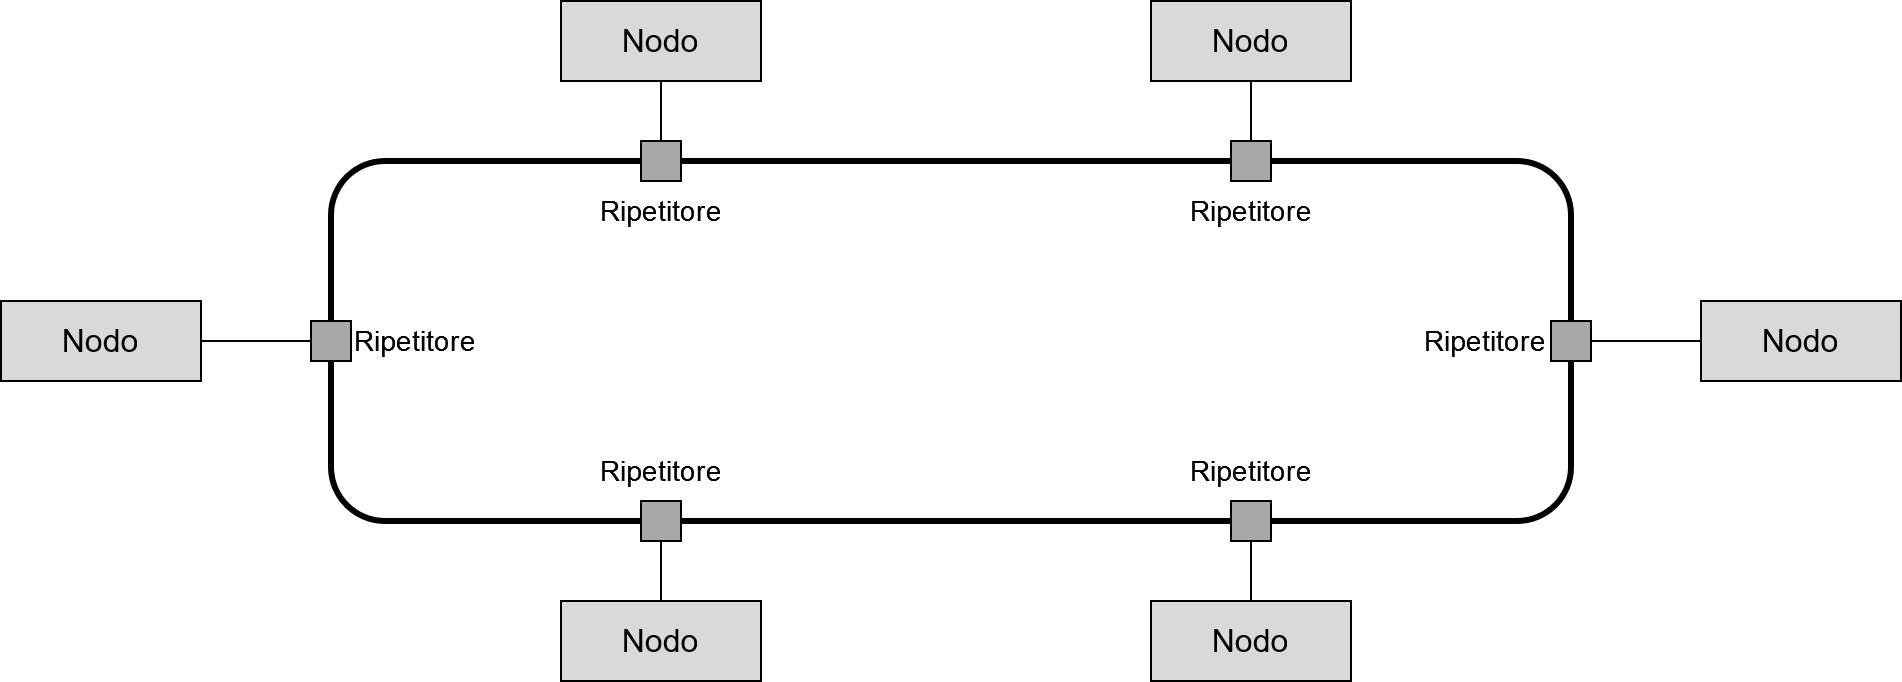
\includegraphics[width=1\textwidth]{img/anello.png}
                \caption{Topologia ad anello.}
                \label{fig:img1}
            \end{figure}
            
            \newpage
            \paragraph{Tipologia ibrida} Chiaramente si può costruire una rete unendo due o più topologie di base.
            
    \subsection{Modelli di rete}
        A causa della grande omogeneità di tecnologie usate per la costruzione di reti, necessitiamo di standard e protocolli per far comunicare due reti eterogenee. I due standard più conosciuti sono il modello OSI (Open System Interconnection) e il modello TCP/IP.
            
        Nel primo l'architettura di una rete è formata da sette livelli, mentre nel modello TCP/IP ne vengono usati cinque.
            
    \subsection{Classificazione delle reti}
        Le reti vengono classificate in base alle loro dimensioni fisiche. Le due categorie principali sono le LAN (Local Area Network) e le WAN (Wide Area Network). La prima ha una dimensione di solitamente non più di due chilometri, mentre la seconda può essere arbitrariamente grande, fino a coprire l'intero globo come accade per Internet. Reti intermedie sono chiamate MAN (Metropolitan Area Network), e spesso ricoprono l'area di un'intera città.
            
        \subsubsection{LAN}
            Una LAN può essere composta anche da soli due computer connessi fra loro, ma solitamente ricopre un edificio o un campus. Le LAN più estese possono collegare più edifici, magari di una stessa compagnia, e connettere dispositivi eterogenei come desktop, stampanti, etc.
                
            Le LAN sono progettate per condividere dati e risorse. Possiamo per esempio immaginare un computer che fa da server e offre accesso (eventualmente controllato) ad applicativi e dati.
                
            Il mezzo trasmissivo è solitamente omogeneo per tutta la rete, e le topologie più utilizzate sono quella a bus, ad anello e a stella.
                
        \subsubsection{WAN}
            Una tale rete mette in comunicazione dispositivi potenzialmente molto lontani, e può essere molto semplice, come nel caso di una connessione punto-punto fra due soli dispositivi, o molto complessa, come nel caso di Internet.
                
            Nel secondo caso di parla di rete WAN a commutazione e la rete è costituita da molti nodi speciali detti router, connessi fra di loro, che collegano le varie reti.
                
        \subsubsection{MAN}
            La dimensione di una Metropolitan Area Network si alloca fra quella di una LAN e di una WAN. Viene tipicamente usata per collegare i vari utenti di una regione, collocati in posizioni diverse, a una rete più grande, tipicamente Internet.
                
    \subsection{Interconnessioni di reti: interreti}
        Oggigiorno è raro trovare una WAN, LAN o MAN isolate da altre reti. Spesso le reti sono connesse ad altre reti, creando interreti o \textbf{internet}.
            
        Abbiamo definito una \textbf{internet} ("i" minuscola) come una qualsiasi rete costruita collegando più reti fra di loro. Ma \textit{Internet} con la "I" maiuscola è la interrete principale e permette a milioni di computer di connettersi fra loro e al World Wide Web.
            
        Storicamente, il protocollo TCP (Transmission Control Protocol) si occupava dello scambio di pacchetti dati, mentre il protocollo IP (Interent Protocol) di operazioni di livello più alto come frammentazione dei pacchetti, consegna affidabile e riassemblaggio. L'unione di questi due protocolli fece nascere il protocollo TCP/IP.
            
    \subsection{Protocolli e standard}
        Un \textbf{protocollo} è un insieme di regole. Affinché le sequenze di bit scambiate fra due nodi di una rete abbiano lo stesso significato per entrambi, serve seguire delle regole. Queste vengono chiamate appunto protocollo, e i suoi elementi chiave sono:
        \begin{itemize}
            \item \textbf{Sintassi.} Definisce il formato dei dati, ossia l'ordine in cui i vari elementi della comunicazione devono essere presentati.
            
            \item \textbf{Semantica.} Definisce il significato delle sequenze di bit.
            
            \item \textbf{Sincronizzazione.} Definisce due aspetti della comunicazione: quando i dati vengono inviati e a che velocità. Queste due caratteristiche devono coincidere altrimenti si rischia di creare un sovraccarico o di perdere dei bit.
        \end{itemize}
        
        Uno standard è comunque un insieme di regole, ma elaborate e approvate da un'organizzazione ufficialmente riconosciuta. Questo è utile se reti diverse o addirittura mutualmente sconosciute vogliono comunicare. Gli standard possono essere:
        \begin{itemize}
            \item \textbf{De facto.} Non sono stati approvati da nessuna organizzazione preposta per tale scopo, ma sono di fatto utilizzati.
            
            \item \textbf{De jure.} Sono stati approvati da un'organizzazione ufficialmente riconosciuta.
        \end{itemize}